\documentclass{article}
\usepackage{tikz}
\usepackage{amsfonts}
\usetikzlibrary{arrows}

\title{Homework \#1}
\author{Kyle White}
\date{February 2, 2017}

\begin{document}
\maketitle

\noindent 0.1)\\
a) This set contains all odd numbers from 1 to $\infty$\\
b) This set contains all even numbers from $-\infty$ to $\infty$\\
c) Any number in the set of Natural numbers that is divisible by 2\\
d) Any number in the set of Natural numbers that is divisible by both 2 and 3\\
e) Any string that is a palindrome made up of 0's and 1's\\
f) Any integer that is equal to 1 added by the input number\\

\noindent 0.2)\\
a) $\left\{1, 10, 100\right\}$\\
b) $\{n \mid n \in \mathbb{Z}, and \ n > 5\}$\\
c) $\{n \mid n \in \mathbb{N}, and \ n > 5\}$\\
d) $\left\{ab\right\}$\\
e) $\left\{ \epsilon \right\}$\\
f) $\emptyset$ \\

\noindent 0.3)\\
a) no\\
b) yes\\
c) $\left\{x,y,z\right\}$\\
d) $\left\{x,y\right\}$\\
e) $\left\{(x,x), (x,y), (y,x), (y,y), (z,x), (z,y)\right\}$\\
f) $\left\{\emptyset, \left\{x\right\}, \left\{y\right\}, \left\{x,y\right\}\right\}$\\

\noindent 0.4) \ There are a*b elements in this set because each element of 'a' must pair with each element of 'b'.  Therefore, there are a*b ordered pairs in this set.
\\ \\
\noindent 0.5) \ There are $2^c$ elements in the power set of C. This is true because each subset of the original set has two subsets of its own that can be derived.  This happens n times until only $\emptyset$ is remaining.  Therefore, there are $2^n$ elements in the power set of a set and, in our case, $2^c$.
\\ \\
\noindent 0.6)\\
a) \ 7
b) \ Range = $\left\{6,7\right\}$, Domain = $\left\{1,5\right\}$\\
c) \ g(2,10) = 6\\
d) \ Range = \{6,10\}, Domain =\{(1,6), (1,7), (1,8), (1,9), (1,10), \\ (2,6), (2,7), (2,8), (2,9), (2,10), \\ (3,6), (3,7), (3,8), (3,9), (3,10), \\ (4,6), (4,7), (4,8), (4,9), (4,10), \\ (5,6), (5,7), (5,8), (5,9), (5,10)\}\\ \\
e) \ g(4, f(4)) = 8\\

\noindent 0.7) \\ \\
a) Two people who have the same mother but different fathers \\
b) x,y \in \mathbb{N} \ and \ x-y \leq 0 \\
c) \ x,y \in \mathbb{Z} \ and \ i*j > 0 \\ \\
\noindent 0.8) \\

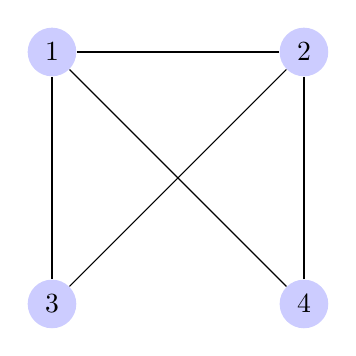
\begin{tikzpicture}
  [scale=.8,auto=left,every node/.style={circle,fill=blue!20}]
	
	\tikzset{
	thick/.style = {line width=1.2pt}
	}
	
  \node (n2) at (0,0) {2};
  \node (n1) at (-4,0)  {1};
  \node (n4) at (0,-4)  {4};
  \node (n3) at (-4,-4) {3};

  \foreach \from/\to in {n1/n2,n1/n3,n1/n4,n2/n3,n2/n4}
    \draw (\from) -- (\to);

\end{tikzpicture}\\ \\

\noindent The path for node 3 to node 4 would go 3--$>$2--$>$4.  I tried to get the graph lines to bold but could not figure it out. \\ \\

\begin{tabular}{l | r}
Node & Degree \\
1 & 3 \\
2 & 3 \\
3 & 2 \\
4 & 2
\end{tabular} \\

\noindent 0.9) \\
G = (V,E)\\
G = $\left\{\left\{1,2,3,4,5,6\right\}, \left\{(1,4), (1,5), (1,6), (2,4), (2,5), (2,6), (3,4), (3,5), (3,6)\right\}\right\}$


\end{document}